\todo{Review comment: Drop Implementation section. [DONE]}

%----------------------------------------------------------------------------------------------------------------
\section{Examples} \label{sec:defeaturing:results}

\todo{Review comment: Drop Results section. Instead take an illustrative part show how it gets defeatured, finally compute effectiveness. [RETAINED THE SECTION. ADDED THE EXAMPLE]}

This section exemplifies the defeaturing approach on a typicall sheet metal part used as ``Electronics Enclosure''.  It is a typical sheet metal casing model used in electronics equipments. 
%%Figure \ref{fig:results:enlosurebenchmark} show the ``Enclosure'' part and its midsurface computed by a commercial application.
%%
%%\def\myfigenlosurebenchmarkcolumnwidth{0.4} %0.466
%%\begin{figure}[!h]
%%\centering     %%% not \center
%%\subfloat[Original Part]{\label{fig:results:originalenclosurepart}\includegraphics[width=\myfigenlosurebenchmarkcolumnwidth\linewidth,valign=t]{../Common/images/SheetMetal_Medium_Enclosure_OriginalPart}} \qquad
%%\subfloat[Commercial Application]{\label{fig:results:midsurfbyinventorexnclosure}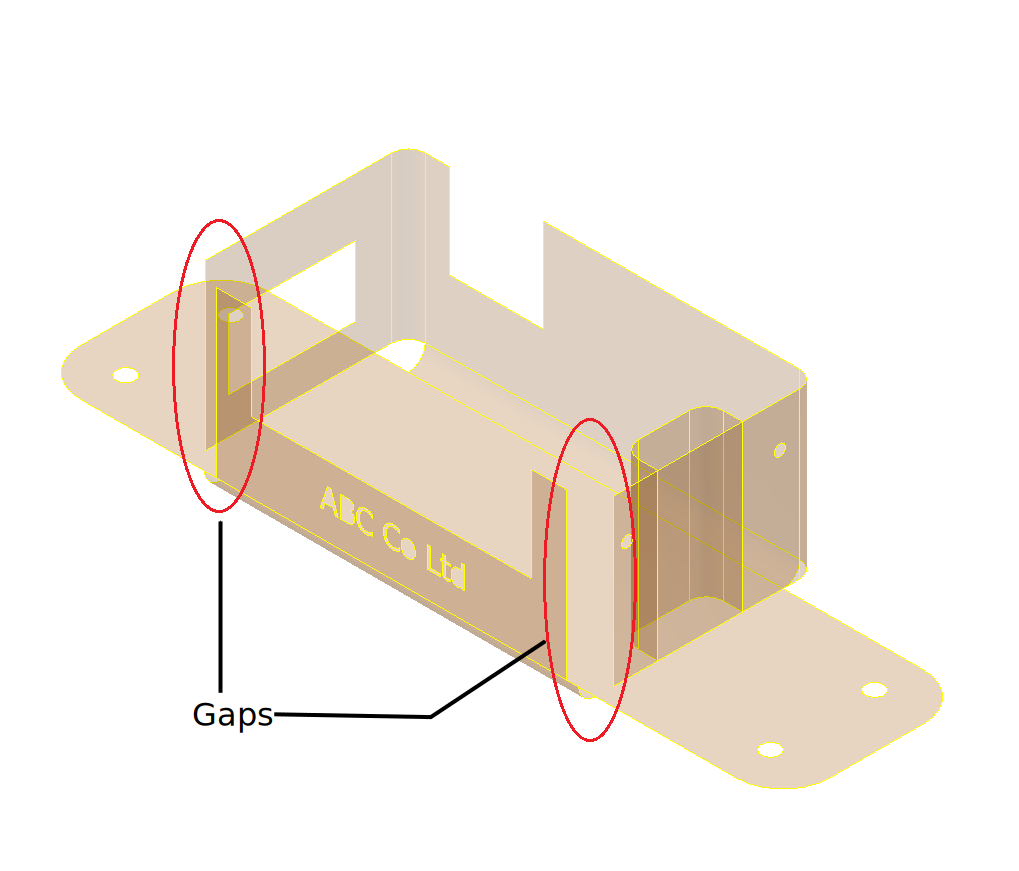
\includegraphics[width=\myfigenlosurebenchmarkcolumnwidth\linewidth,valign=t]{../Common/images/SheetMetal_Medium_Enclosure_InventorMidsurfwithErrors}}
%%\caption{Computation of Midsurface of an Enclosure Model}
%%\label{fig:results:enlosurebenchmark}
%%\end{figure}
%%
%%Quite a few failures are seen, such as disconnected patches, missing midsurface patches etc. Following sections show progress of the part while goring through various modules.


Following are the steps through which defeaturing of ``Enclosure'' happens. The threshold (D) taken here is 5\%.

%\begin{enumerate}
%[noitemsep,topsep=2pt,parsep=2pt,partopsep=2pt]
%\item
%The model has 3 cutouts for components interfacing with outside world, letter embossing, a chute for wires and holes for fixing bolts.


%%\bigskip

%\begin{figure}[!h]
%\centering     %%% not \center
%\subfloat[Input CAD Model]{\label{fig_enclinputmodel}\includegraphics[width=0.62\linewidth,valign=t]{../Common/images/SheetMetal_Medium_Enclosure_OriginalPart}} \qquad
%\subfloat[Feature Tree]{\label{fig_enclinputree}\includegraphics[width=0.32\linewidth,valign=t]{../Common/images/SheetMetal_Medium_Enclosure_OriginalTree}}
%\caption{Input CAD Model with Its Feature Tree}
%\label{fig:results:examples1cad}
%\end{figure}


\begin{minipage}{\linewidth}
\begin{minipage}[c]{0.62\linewidth}
\includegraphics[width=\linewidth,valign=t]{../Common/images/SheetMetal_Medium_Enclosure_OriginalPart}
%\captionof{figure}{Input CAD Model} \label{fig_enclinputmodel}
\captionof{figure}{Input CAD Model} \label{fig_enclinputmodel}

\bigskip

 Figure \ref{fig_enclinputmodel} shows the input Enclosure part model its corresponding feature tree. It is modeled in Autodesk Inventor using sheet metal features such as Face(Wall), Flange, Bend, Emboss, array of Slots, etc. 
 
\end{minipage}
\hfill
\begin{minipage}[c]{0.32\linewidth}
\includegraphics[width=\linewidth,valign=t]{../Common/images/SheetMetal_Medium_Enclosure_OriginalTree}
%\captionof{figure}{Feature Tree} \label{fig_enclinputree}
\end{minipage}

\end{minipage}

%%\bigskip


%\item 

\begin{minipage}{\linewidth}
\begin{minipage}[c]{0.62\linewidth}
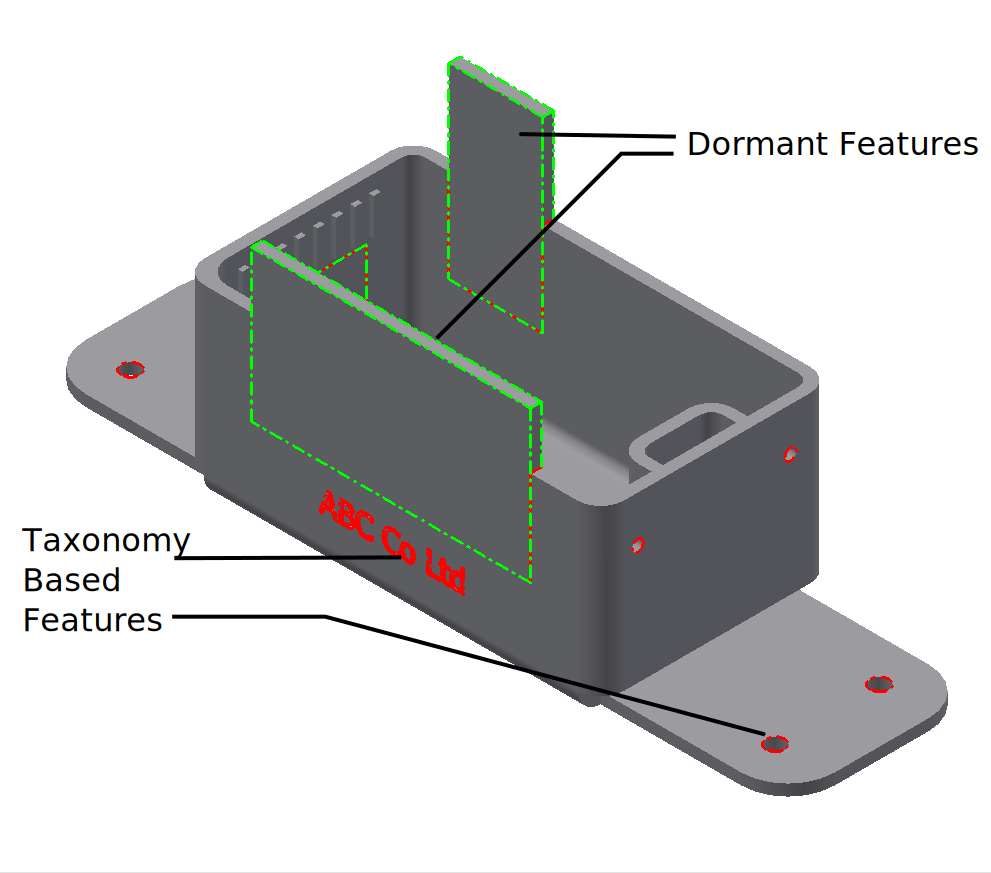
\includegraphics[width=\linewidth,valign=t]{../Common/images/SheetMetal_Medium_Enclosure_PhaseISelections_2}
%\captionof{figure}{Detected Features Shown in Model} \label{fig_enclph1model}

\captionof{figure}{Features Identified for Removal Shown in Model and Tree} \label{fig_enclph1model}

\bigskip

Figure \ref{fig_enclph1model} shows the selection of irrelevant sheet metal features based on newly proposed sheet metal feature taxonomy  (in red color). It also shows the bulk negative features as dormant features (in green).  %Figure \ref{fig_enclph1tree} shows the selections in the feature tree.

\end{minipage}
\hfill
\begin{minipage}[c]{0.32\linewidth}
\includegraphics[width=\linewidth,valign=t]{../Common/images/SheetMetal_Medium_Enclosure_PhaseISelectionsTree}
%\captionof{figure}{Detected Features Shown in Tree} \label{fig_enclph1tree}
\end{minipage}

\end{minipage}


%\item 

\begin{minipage}{\linewidth}
\begin{minipage}[c]{0.62\linewidth}
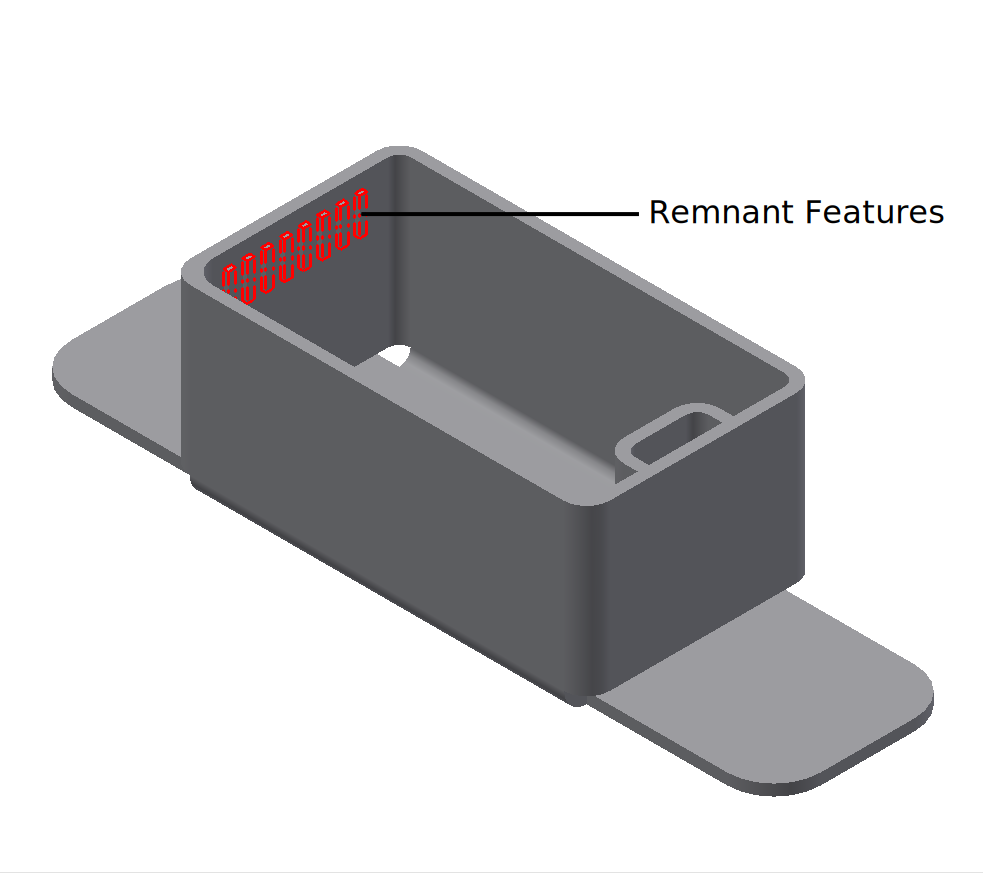
\includegraphics[width=\linewidth,valign=t]{../Common/images/SheetMetal_Medium_Enclosure_PhaseIISelections_2}

\captionof{figure}{Removal of Features Based on Remnant Feature Approach} \label{fig_enclph2model}

\bigskip

Figure \ref{fig_enclph2model} shows (in red color) the selection of irrelevant sheet metal features based on remnant feature portions.% Figure \ref{fig_enclph2tree} shows same selections in the feature tree.

\end{minipage}
\begin{minipage}[c]{0.32\linewidth}
\includegraphics[width=\linewidth,valign=t]{../Common/images/SheetMetal_Medium_Enclosure_PhaseIISelectionsTree}
%\captionof{figure}{Detected Remnant Features Shown in Tree} \label{fig_enclph2tree}
\end{minipage}

\end{minipage}

%%\bigskip


%\item 
\begin{minipage}{\linewidth}
\begin{minipage}[c]{0.62\linewidth}
\includegraphics[width=\linewidth,valign=t]{../Common/images/SheetMetal_Medium_Enclosure_DefeaturedPart}
%\captionof{figure}{Output Gross Shape} \label{fig_Defeaturedmodel}

\captionof{figure}{CAD Model after Full Defeaturing} \label{fig_Defeaturedmodel}

\bigskip

Figure \ref{fig_Defeaturedmodel} shows the result of defeaturing process along with the feature tree. The model has been simplified substantially (\~75\% reduction in the number of faces) while retaining all the principal features thus preserving the gross shape intent.

\end{minipage}
\begin{minipage}[c]{0.32\linewidth}
\includegraphics[width=\linewidth,valign=t]{../Common/images/SheetMetal_Medium_Enclosure_DefeaturedTree}
%\captionof{figure}{Features Removed} \label{fig_Defeaturedtree}
\end{minipage}

\end{minipage}

%%\bigskip


%%\def\myfigenlosuredefeaturecolumnwidth{0.95}
%%\def\myfigenlosuredefeatureTreecolumnwidth{0.75}
%%\begin{longtable}[h]{@{} p{0.18\linewidth}  p{0.38\linewidth} p{0.1\linewidth} p{0.2\linewidth}@{}}
%%\toprule
%% & Model & Tree & Explanation \\
%% \midrule
%% 
%%Original/Input &
%%\raisebox{-0.8\height}{\includegraphics[width=\myfigenlosuredefeaturecolumnwidth\linewidth]{..//Common/images/SheetMetal_Medium_Enclosure_OriginalPart}} &
%%\raisebox{-0.8\height}{\includegraphics[width=\myfigenlosuredefeatureTreecolumnwidth\linewidth]{..//Common/images/SheetMetal_Medium_Enclosure_OriginalTree}} &
%%
%%The model has 3 cutouts for components interfacing with outside world, letter embossing, a chute for wires and holes for fixing bolts.\\
%%
%%Phase I Selections &
%%\raisebox{-0.8\height}{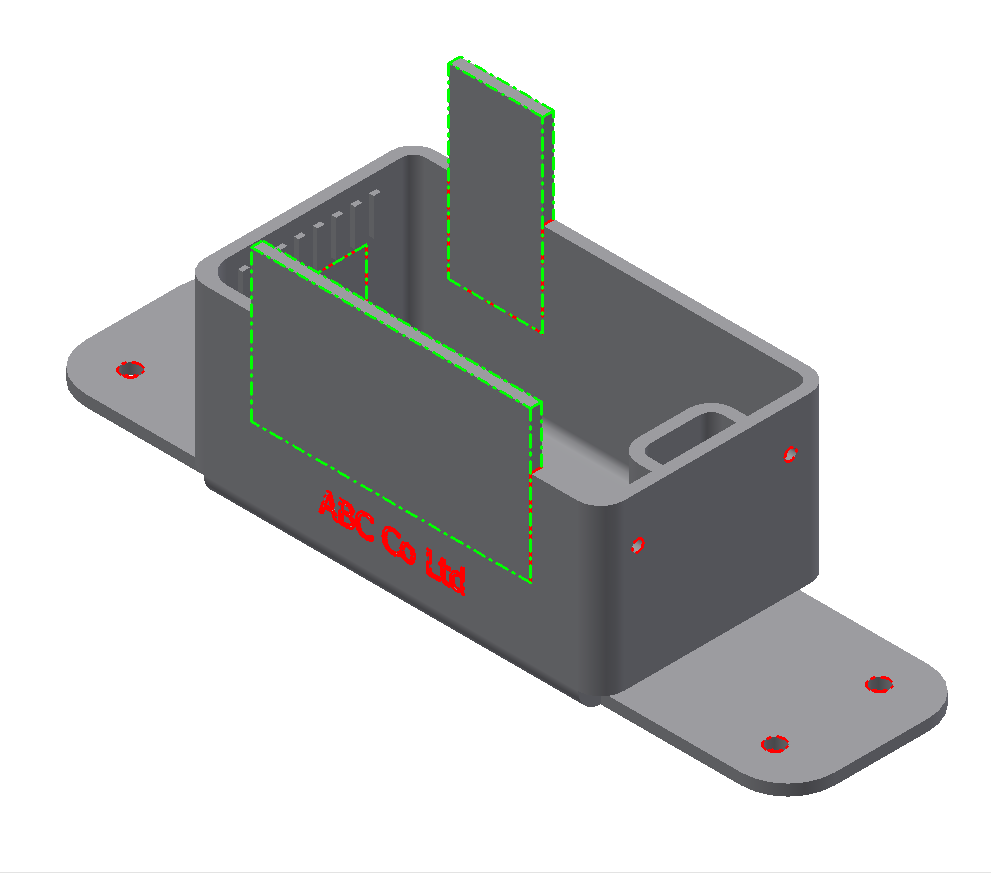
\includegraphics[width=\myfigenlosuredefeaturecolumnwidth\linewidth]{..//Common/images/SheetMetal_Medium_Enclosure_PhaseISelections}} &
%%\raisebox{-0.8\height}{\includegraphics[width=\myfigenlosuredefeatureTreecolumnwidth\linewidth]{..//Common/images/SheetMetal_Medium_Enclosure_PhaseISelectionsTree}} &
%%
%%Small holes, emobssing is chosen based on Sheet Metal feature taxonomy rules (shown red). The green selections are the dormant feature bodies cached.\\
%%
%%Phase II  Selections&
%%\raisebox{-0.8\height}{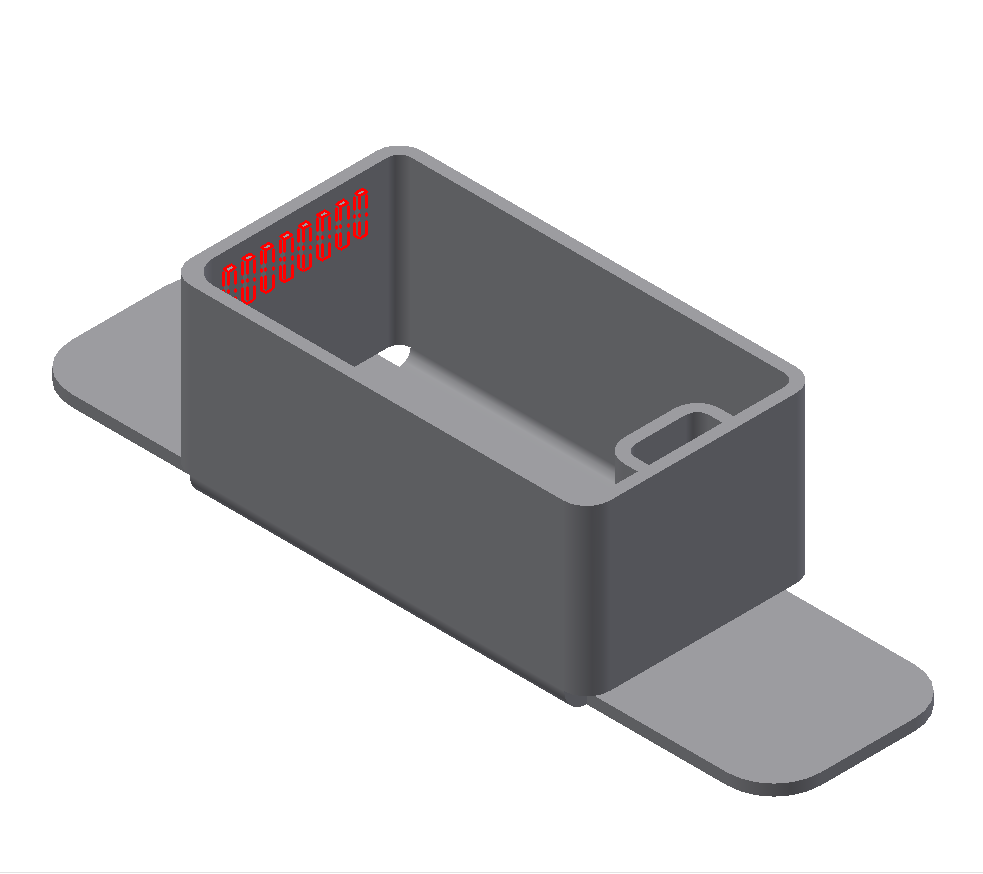
\includegraphics[width=\myfigenlosuredefeaturecolumnwidth\linewidth]{..//Common/images/SheetMetal_Medium_Enclosure_PhaseIISelections}} &
%%\raisebox{-0.8\height}{\includegraphics[width=\myfigenlosuredefeatureTreecolumnwidth\linewidth]{..//Common/images/SheetMetal_Medium_Enclosure_PhaseIISelectionsTree}} &
%%
%%Remnant features got selected in the second phase. \\
%%
%%Defeatured&
%%\raisebox{-0.8\height}{\includegraphics[width=\myfigenlosuredefeaturecolumnwidth\linewidth]{..//Common/images/SheetMetal_Medium_Enclosure_DefeaturedPart}} &
%%\raisebox{-0.8\height}{\includegraphics[width=\myfigenlosuredefeatureTreecolumnwidth\linewidth]{..//Common/images/SheetMetal_Medium_Enclosure_DefeaturedTree}} &
%%
%%Most of the unnecessary features are removed and now it retains all the necessary features adequately ``representing''  the gross shape. \\
%%
%%\bottomrule
%%\end{longtable}

%\item 
Effectiveness with 5\% threshold, based on the criterion defined by Eqn. \ref{eqn:defeaturing:effectiveness} is:

\begin{minipage}[c]{0.98\linewidth}
\captionof{table}{Defeaturing Effectiveness Data} \label{tbl_defeatdata}
\begin{longtable}[h]{@{} p{0.3\linewidth} |p{0.3\linewidth}| p{0.3\linewidth} @{}}\toprule
\textbf{Number of Faces Before Defeaturing } & \textbf{Number of Faces {remaining} after Taxonomy-Size Based Defeaturing} & \textbf{Number of Faces {remaining} at the End}\\  \midrule
259 & 104 & 64\\
%  &13 & 8\\
\bottomrule
\end{longtable}

\end{minipage}

\bigskip

\begin{equation}
pR = (1 - \frac{64}{259}) \times 100 = 75.29\%
\label{eqn_case1}
\end{equation}

%\end{enumerate}

%%\bigskip

Table~\ref{tbl_defeatdata} shows the data collected at each phase. It can be seen that even after huge reduction in the number of faces (75\% seen in Eqn.~\ref{eqn_case1}), the overall shape of the enclosure is retained appropriately. This defeatured model is sent for further processing to compute a quality midsurface.

Following section presents conclusions of the process of investigation of problems and proposing solution for defeaturing a sheet metal feature based CAD model.



%%Uniqueness of the present research work with respect to some other relevant approaches \cite{Kannan2009,SangHunLee2005,Russ2012}:
%%	\begin{itemize}
%%	[noitemsep,topsep=2pt,parsep=2pt,partopsep=2pt]
%%	\item Suppressibility rules specific to the domain such as sheet metal feature based design. 
%%	\item Suppressibility rules based on the remnant and not full feature/part volume.
%%	\item No blind suppression of all the negative features or filling-up of the concave volumes.
%%\end{itemize}
%%%%\bigskip

%%Following test cases show the effect of defeaturing on the quality of the midsurface. Size threshold used here is certain percentage of the summation of face-areas of all the faces in the original body.
%%
%%\begin{enumerate}
%%\item Threshold (D) 3\% of the total part size
%%
%%
%%\begin{tabular}[h]{@{} p{0.12\linewidth}  p{0.28\linewidth} p{0.28\linewidth} p{0.28\linewidth}@{}}
%%\toprule
%% & Model & Midsurface & Explanation \\
%% \midrule
%% 
%%Original input &
%%\raisebox{-0.8\height}{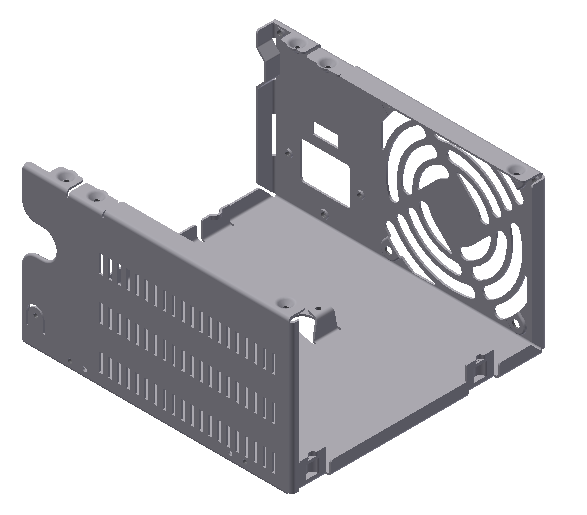
\includegraphics[width=0.8\linewidth]{..//Common/images/defeatresult_perc3_origpart}} &
%%\raisebox{-0.8\height}{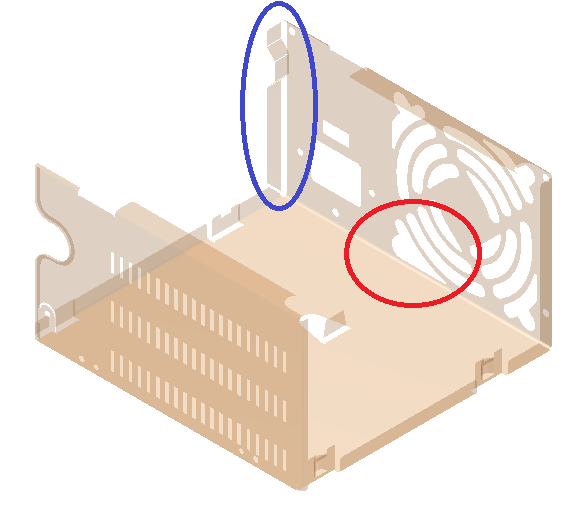
\includegraphics[width=0.8\linewidth]{..//Common/images/defeatresult_perc3_origmids}} &
%%Gaps in the midsurface. Two of the gaps are marked (blue and red).\\
%%
%%Output of Phase I and input to Phase II &
%%\raisebox{-0.8\height}{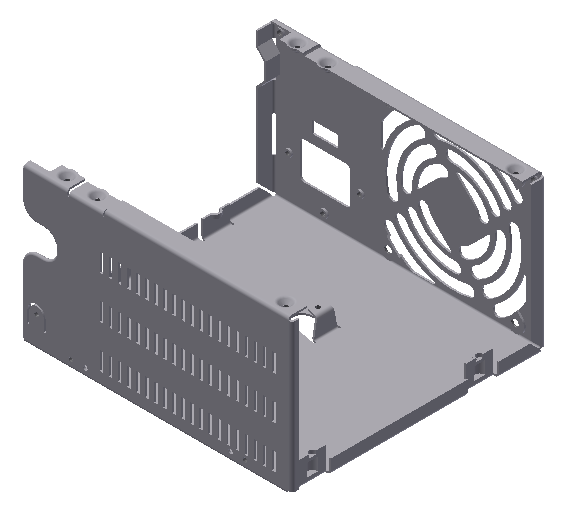
\includegraphics[width=0.8\linewidth]{..//Common/images/defeatresult_perc3_ph1part}} &
%%\raisebox{-0.8\height}{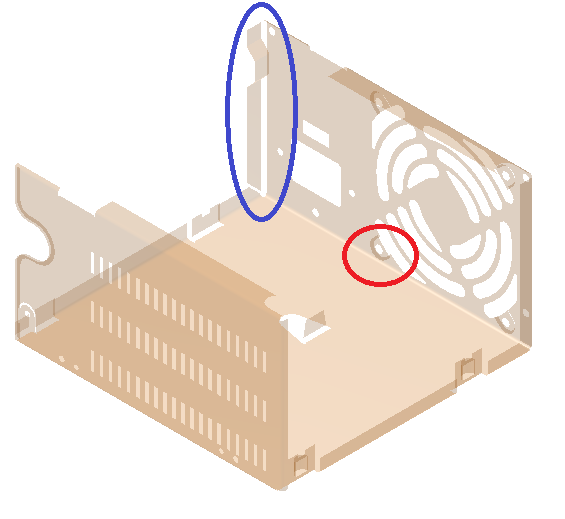
\includegraphics[width=0.8\linewidth]{..//Common/images/defeatresult_perc3_ph1mids}} &
%%Although the number of gaps have reduced (the red gap is filled), but the gaps between the surface patches (blue gap) is still seen. \\
%%
%%Output of Phase II &
%%\raisebox{-0.8\height}{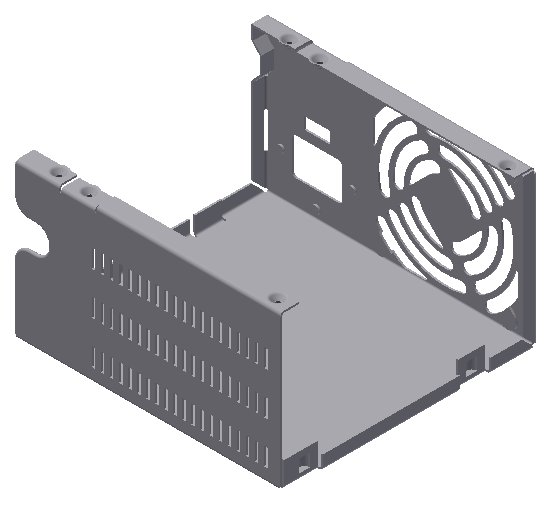
\includegraphics[width=0.8\linewidth]{..//Common/images/defeatresult_perc3_ph2part}} &
%%\raisebox{-0.8\height}{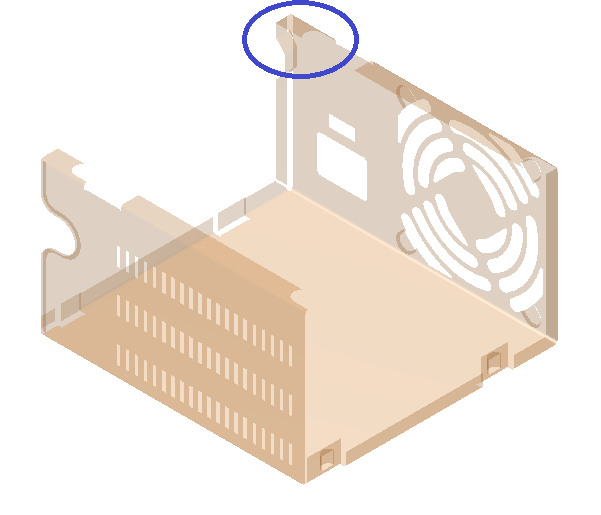
\includegraphics[width=0.8\linewidth]{..//Common/images/defeatresult_perc3_ph2mids}} &
%%Some of the gaps (blue gap top portion) are filled and the output is a bit better-connected midsurface. \\
%%
%%\bottomrule
%%\end{tabular}
%%
%%Effectiveness of Smarf with 3\% threshold by Eqn. \ref{eqn:defeaturing:effectiveness} is:
%%
%%\begin{minipage}[c]{0.6\linewidth}
%%\begin{tabular}[h]{@{} p{0.22\linewidth} p{0.18\linewidth} p{0.21\linewidth} p{0.2\linewidth} @{}}\toprule
%%\textbf{Qty} & \textbf{Input} & \textbf{Phase I} & \textbf{Output}\\  \midrule
%%Faces  & 1434 & 610 & 327\\
%%Suppressed  &  & 60 & 30\\
%%\bottomrule
%%\end{tabular}
%%\end{minipage}
%%\begin{minipage}[c]{0.38\linewidth}
%%$pR = (1 - \frac{697}{833}) \times 100 = 16\%$
%%\end{minipage}
%%
%%
%%\item Threshold (D) 5\% of the total part size
%%
%%
%%\begin{tabular}[h]{@{} p{0.12\linewidth}  p{0.28\linewidth} p{0.28\linewidth} p{0.28\linewidth}@{}}
%%\toprule
%% & Model & Midsurface & Explanation \\
%% \midrule
%% 
%%Original input&
%%\raisebox{-0.8\height}{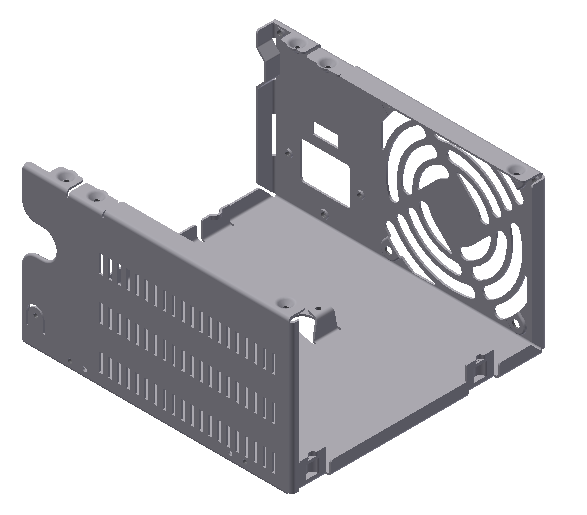
\includegraphics[width=0.8\linewidth]{..//Common/images/defeatresult_perc5_origpart}} &
%%\raisebox{-0.8\height}{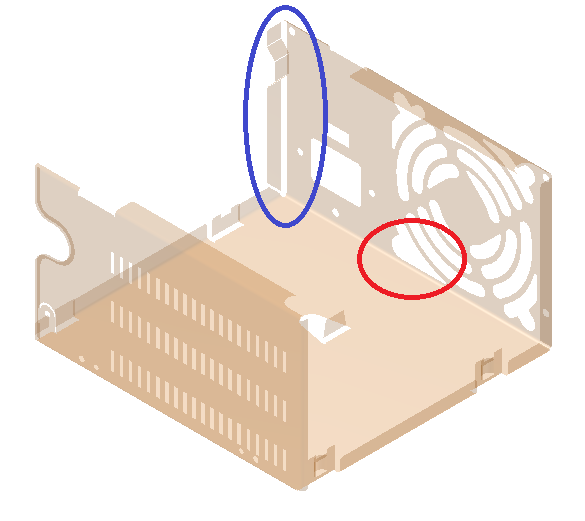
\includegraphics[width=0.8\linewidth]{..//Common/images/defeatresult_perc5_origmids}} &
%%Gaps in the midsurface. Two of the gaps are marked (blue and red).\\
%%
%%Output of Phase I and input to Phase II &
%%\raisebox{-0.8\height}{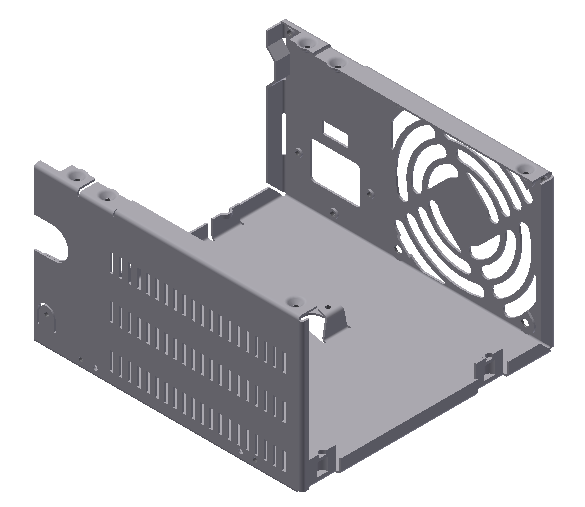
\includegraphics[width=0.8\linewidth]{..//Common/images/defeatresult_perc5_ph1part}} &
%%\raisebox{-0.8\height}{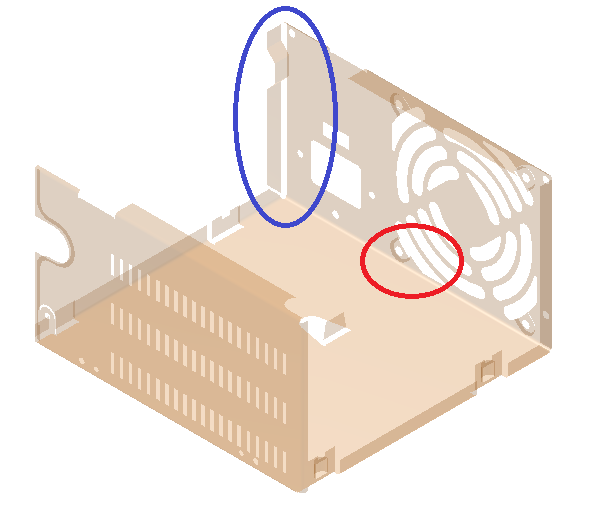
\includegraphics[width=0.8\linewidth]{..//Common/images/defeatresult_perc5_ph1mids}} &
%%Although the number of missing gaps in the midsurface has reduced (red gap is filled), but the gaps between the surface patches (blue gap) is still seen.\\
%%
%%Output of Phase II &
%%\raisebox{-0.8\height}{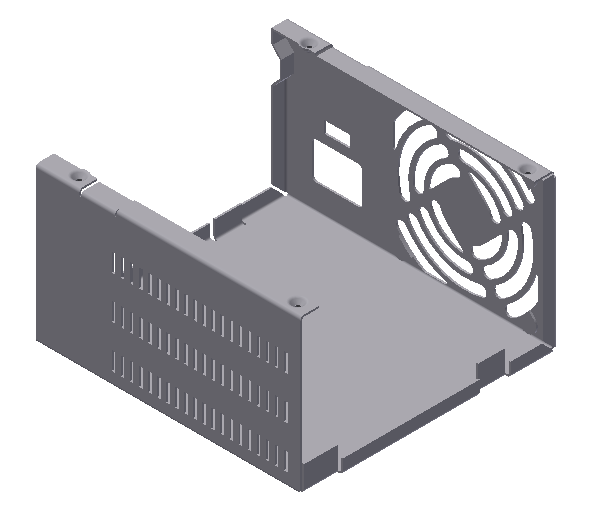
\includegraphics[width=0.8\linewidth]{..//Common/images/defeatresult_perc5_ph2part}} &
%%\raisebox{-0.8\height}{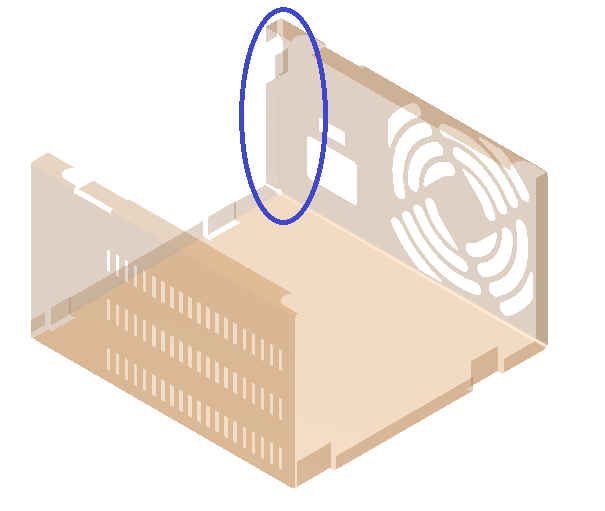
\includegraphics[width=0.8\linewidth]{..//Common/images/defeatresult_perc5_ph2mids}} &
%%Most of the gaps (blue gap full) are filled and the output is a better-connected midsurface. It retains all the necessary features adequately ``representing''  the gross shape. \\
%%
%%\bottomrule
%%\end{tabular}
%%
%%Effectiveness of Smarf with 5\% threshold by Eqn. \ref{eqn:defeaturing:effectiveness} is:
%%
%%\begin{minipage}[c]{0.6\linewidth}
%%\begin{tabular}[h]{@{} p{0.22\linewidth} p{0.18\linewidth} p{0.21\linewidth} p{0.2\linewidth} @{}}\toprule
%%\textbf{Qty} & \textbf{Input} & \textbf{Phase I} & \textbf{Output}\\  \midrule
%%Faces  & 833 & 772 & 617\\
%%Suppressed  &  &7 & 40\\
%%\bottomrule
%%\end{tabular}
%%\end{minipage}
%%\begin{minipage}[c]{0.38\linewidth}
%%$pR = (1 - \frac{697}{833}) \times 100 = 26\%$
%%\end{minipage}
%%
%%\item Threshold (D) 10\% of the total part size
%%
%%
%%\begin{tabular}[h]{@{} p{0.12\linewidth}  p{0.28\linewidth} p{0.28\linewidth} p{0.28\linewidth}@{}}
%%\toprule
%% & Model & Midsurface & Explanation \\
%% \midrule
%% 
%%Original input  &
%%\raisebox{-0.8\height}{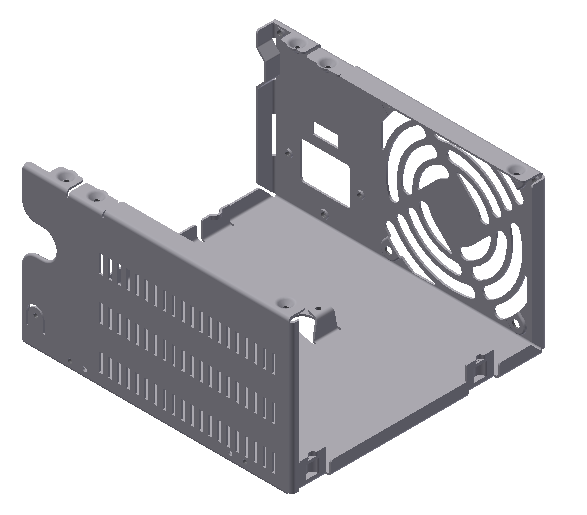
\includegraphics[width=0.8\linewidth]{..//Common/images/defeatresult_perc10_origpart}} &
%%\raisebox{-0.8\height}{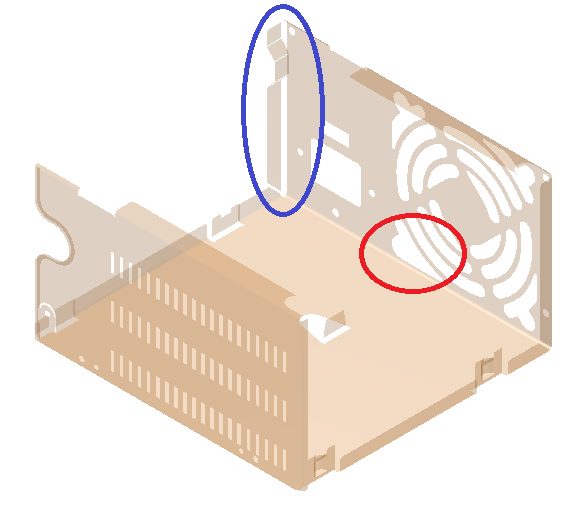
\includegraphics[width=0.8\linewidth]{..//Common/images/defeatresult_perc10_origmids}} &
%%Gaps in the midsurface. Two of the gaps are marked (blue and red).\\
%%
%%Output of Phase I and input to Phase II &
%%\raisebox{-0.8\height}{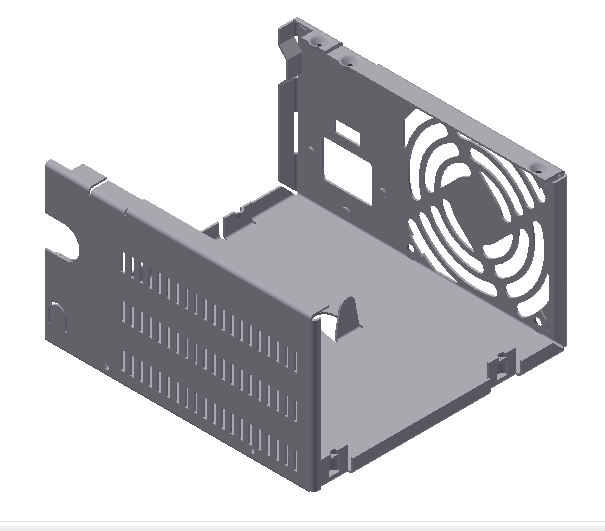
\includegraphics[width=0.8\linewidth]{..//Common/images/defeatresult_perc10_ph1part}} &
%%\raisebox{-0.8\height}{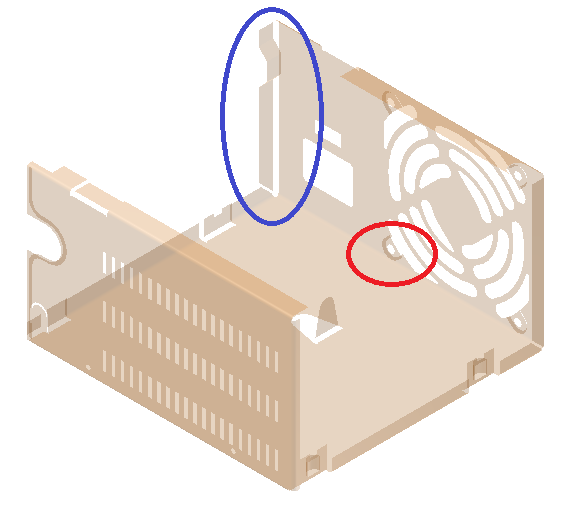
\includegraphics[width=0.8\linewidth]{..//Common/images/defeatresult_perc10_ph1mids}} &
%%Although the number of missing gaps in the midsurface has reduced (red gap is filled), but the gaps between the surface patches (blue gap) is still seen. \\
%%
%%Output of Phase II &
%%\raisebox{-0.8\height}{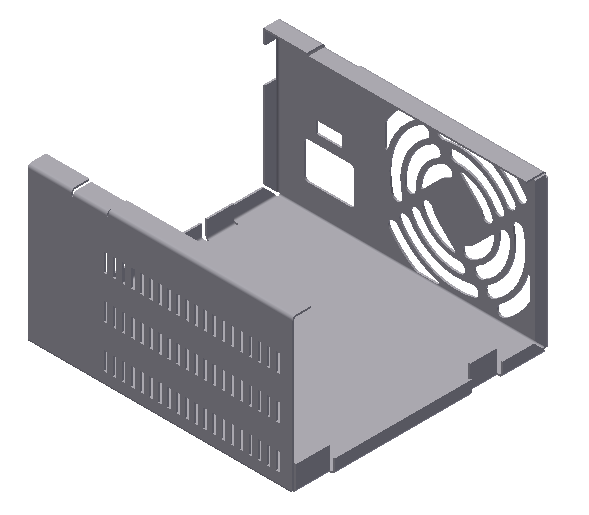
\includegraphics[width=0.8\linewidth]{..//Common/images/defeatresult_perc10_ph2part}} &
%%\raisebox{-0.8\height}{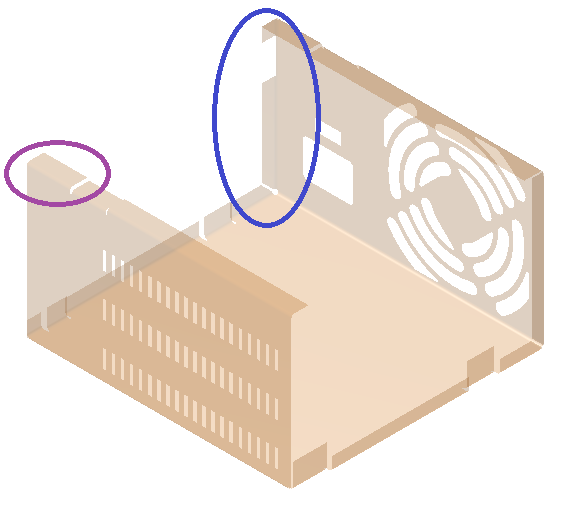
\includegraphics[width=0.8\linewidth]{..//Common/images/defeatresult_perc10_ph2mids}} &
%%Most of the gaps (blue gap full) are filled. Removal of purple feature could be the domain decision. It retains all the necessary features adequately ``representing''  the gross shape. \\
%%
%%\bottomrule
%%\end{tabular}
%%
%%Effectiveness of Smarf with 10\% threshold by Eqn. \ref{eqn:defeaturing:effectiveness} is:
%%
%%\begin{minipage}[c]{0.6\linewidth}
%%\begin{tabular}[h]{@{} p{0.22\linewidth} p{0.18\linewidth} p{0.21\linewidth} p{0.2\linewidth} @{}}\toprule
%%\textbf{Qty} & \textbf{Input} & \textbf{Phase I} & \textbf{Output}\\  \midrule
%%Faces  & 833 & 715 & 522\\
%%Suppressed  &  &17 & 48\\
%%\bottomrule
%%\end{tabular}
%%\end{minipage}
%%\begin{minipage}[c]{0.38\linewidth}
%%$pR = (1 - \frac{522}{833}) \times 100 = 37\%$
%%\end{minipage}
%%\end{enumerate}
%%
%%The choice of threshold can be set to such a value where midsurface output is well-connected. In the test-cases shown above 10\% appears to be the appropriate value. Increasing the threshold to still higher value results in a well-connected midsurface but it loses the shape characteristics which need to be maintained (Table \ref{tbl:litsurvey:defeatmids}).
